\documentclass{article}

\usepackage{amsthm}
\newtheorem{proposition}{Proposition}[section]
\theoremstyle{definition}
\newtheorem{definition}{Definition}[section]
\newtheorem{theorem}{Theorem}[section]
\newtheorem{example}{Example}[section]
\theoremstyle{remark}
\newtheorem{remark}{Remark}[section]
\newtheorem{lemma}{Lemma}[section]

\setlength{\parskip}{0.5em}

\usepackage{multicol}
\usepackage[linesnumbered,ruled,vlined]{algorithm2e}
\usepackage{comment}
\usepackage{pgf}
\usepackage{tikz}
\usetikzlibrary{arrows,automata}
\usepackage[utf8]{inputenc} 		% encodage des caracteres utilise (pour les caracteres accentues) -- non utilise ici.
%\usepackage[latin1]{inputenc} 		% autre encodage
\usepackage[english]{babel}		% pour une mise en forme "anglaise"
\usepackage{amsmath,amssymb,amsthm}	% pour les maths
\usepackage{graphicx}			% pour inclure des graphiques
\usepackage{hyperref}			% si vous souhaitez que les references soient des hyperliens
\usepackage{color}			% pour ajouter des couleurs dans vos textes
\usepackage{todonotes}

\def \N {\mathbb N}	

\newcommand{\TodoDavid}[1]{\todo[color=green!40]{#1}}
\newcommand{\TodoJF}[1]{\todo{#1}}

\newcommand{\Vars}{\textbf{Vars}}
\newcommand{\MC}{\textbf{MC}}
\newcommand{\Terms}{\textbf{Terms}}
\newcommand{\Preds}{\textbf{Preds}}
\newcommand{\Csts}{\textbf{Csts}}
\newcommand{\Merge}{\textit{Merge}}
\newcommand{\Depth}{\textit{depth}}
\newcommand{\Appl}{\textbf{appl}}
\newcommand{\father}{\textbf{father}}
\newcommand{\Tree}{\textit{Tree}}
\newcommand{\Fut}{\textbf{Fut}}
\newcommand{\des}{\textbf{Desc}}
\newcommand{\ALCH}{\textbf{Horn-$\mathcal{ALCH}$}}
\newcommand{\ALCHI}{\textbf{Horn-$\mathcal{ALCHI}$}}

\title{Implementing the Core Chase for $\ALCH$}
\author{Maël Abily}	


\begin{document}
\maketitle						% Genere le titre



\section{Introduction}

The conjunctive query entailment is an important issue in knowledge representation. This problem can be described in a first order logic background. We work on conjunctive formulas (that are formulas constructed only with conjunction and existential quantification) and queries that are conjunctive formulas without free variables; the answer of a query is either yes or no. For example $ \exists y. \textit{Human}(y) \wedge \textit{IsTheBrotherOf}(\textbf{Pierre},y)$ is a query asking
if Pierre has a parent. We also work on existential rules that are formulas of the form $\forall \vec x.\forall \vec y.( A(\vec x,\vec y) \rightarrow \exists \vec z. B(\vec x,\vec z))$ where $\vec u$ represents a tuple of variables. A theory $T$ will then be a set of existential rules and conjunctive formulas

We can now define the problem of conjunctive query entailment: Given a theory $T$ and a query $Q$ determine if $T$ entails the query $Q$. For example, the set $T= \{\textit{IsTheBrotherOf}(\textbf{Pierre},\textbf{Marie}),$ $\forall x \forall y. \textit{IsTheBrotherOf}(x,y) \rightarrow \textit{Human}(x) \wedge \textit{Human}(y) \}$ entails the query $Q=\exists y. \textit{Human}(y) \wedge \textit{IsTheBrotherOf}(\textbf{Pierre},y)$.



We usually use reasoning algorithms to answer the conjunctive query entailment. Note that in practice, a lot of formulas can be expressed via conjunctive formulas. By definition, a theory $T$ entails a query $Q$ if every  model of $T$ is a model of $Q$. However, we cannot compute all models because $T$ can have an infinite number of models.

To deal with this problem, we can compute an\todo{a}\ universal model of the theory $T$. That is a model of $T$ that is entailed by all the models of $T$. If a such model $U$ exists, we just need to show that $U$ entails $Q$ to conclude that $T$ entails $Q$. Hence, to solve query entailment, we just have to compute a finite universal model $U$ for a given input $T$ and check if $U$ entails $Q$.

To compute these models, we can use the chase. In this document, we present several variants of this algorithm: the oblivious chase, the restricted chase and then the core chase. The last chase is the best in the sense it is the only one that terminates if and only if there exists a finite universal model.

Nevertheless, the core chase is more complicated to implement because . \todo{Maybe explain a bit why is it hard to implement?} We will then focus on a restricted type of theory $T$ (that is called \ALCH\ theory) where the set of conjunctive formulas is ground (that is there is no free-variable in the formula) and where the rules contained in $T$ are \ALCH\ axioms.\todo{Explain why \ALCH is interesting: talk a bit about description logics.}

We present a new variant of the chase for \ALCH\ theories which is also guaranteed to terminate if the input theory admits a finite universal model and is much easier to implement. In the core chase, one has to look for global endomorphisms in the sets of facts produced by the chase whereas in the merge chase, we only need to look for very local endomorphisms, which are much simpler to compute.

\begin{figure}
\begin{center}
\begin{tikzpicture}[scale=0.2]
\tikzstyle{every node}+=[inner sep=0pt]

\draw [white] (17.1,-35.9) circle (3);
\draw (17.1,-35.9) node {$a$};
\draw [white] (10.1,-24.1) circle (3);
\draw (10.1,-24.1) node {$t$};
\draw [white] (24.1,-24.1) circle (3);
\draw (24.1,-24.1) node {$y$};
\draw [white] (24.1,-12.4) circle (3);
\draw (24.1,-12.4) node {$x$};
\draw [white] (10.1,-12.4) circle (3);
\draw (10.1,-12.4) node {$z$};
\draw [white] (30.7,-24.6) circle (3);
\draw [white] (50.4,-24.6) circle (3);
\draw [white] (59.7,-36.8) circle (3);
\draw (59.7,-36.8) node {$a$};
\draw [white] (59.7,-25.3) circle (3);
\draw (59.7,-25.3) node {$t$};
\draw [white] (53.4,-13.2) circle (3);
\draw (53.4,-13.2) node {$z$};
\draw [white] (65.4,-13.2) circle (3);
\draw (65.4,-13.2) node {$x$};
\draw [black] (15.57,-33.32) -- (11.63,-26.68);
\fill [black] (11.63,-26.68) -- (11.61,-27.62) -- (12.47,-27.11);
\draw (14.25,-28.75) node [right] {};
\draw [black] (10.1,-21.1) -- (10.1,-15.4);
\fill [black] (10.1,-15.4) -- (9.6,-16.2) -- (10.6,-16.2);
\draw (10.6,-18.25) node [right] {};
\draw [black] (18.63,-33.32) -- (22.57,-26.68);
\fill [black] (22.57,-26.68) -- (21.73,-27.11) -- (22.59,-27.62);
\draw (21.25,-31.25) node [right] {};
\draw [black] (24.1,-21.1) -- (24.1,-15.4);
\fill [black] (24.1,-15.4) -- (23.6,-16.2) -- (24.6,-16.2);
\draw (24.6,-18.25) node [right] {};
\draw [black] (33.7,-24.6) -- (47.4,-24.6);
\fill [black] (47.4,-24.6) -- (46.6,-24.1) -- (46.6,-25.1);
\draw [black] (59.7,-33.8) -- (59.7,-28.3);
\fill [black] (59.7,-28.3) -- (59.2,-29.1) -- (60.2,-29.1);
\draw (60.2,-31.05) node [right] {};
\draw [black] (58.31,-22.64) -- (54.79,-15.86);
\fill [black] (54.79,-15.86) -- (54.71,-16.8) -- (55.6,-16.34);
\draw (57.24,-18.11) node [right] {};
\draw [black] (60.98,-22.59) -- (64.12,-15.91);
\fill [black] (64.12,-15.91) -- (63.33,-16.42) -- (64.23,-16.85);
\draw (63.26,-20.3) node [right] {};
\end{tikzpicture}
\end{center}
\label{figure:intro}
\caption{Merging Example}
\end{figure}



\tableofcontents			

First of all, we will define the usefull notions for this paper and give some well known properties. Then, we will move on our contributions. 

\section{Background}


\subsection{Facts}

\subsubsection{Syntax}

We consider a set of variables \Vars, a set of constants \Csts, and a set of predicates \Preds, that are pairwise disjoint. A \emph{term} is a variable or a constant. We note \Terms\ the set of terms. If $t_1,\ldots,t_n$ are terms and $P$ is a predicate of arity $n$, then $P(t_{1},\ldots,t_{n})$ is an \emph{atom}. The atom $P(t_{1},\ldots,t_{n})$ is \emph{ground} if $t_1,\ldots,t_n$ are constants. We can now define a factbase that is a notion omnipresent in all the paper.  


\begin{definition}
A \emph{factbase} $F$ is an existentially closed conjunction of atoms, that is, a formula that does not contain occurrences of free variables and is of the form $\exists x_{1},\ldots,x_{n}.P_{1}(t_{1}^{1},\ldots,t_{k_{1}}^{1})\land \ldots\land P_{m}(t_{1}^{m},\ldots,t_{k_{m}}^{m})$ where $t_i^j$ are terms and $P_i$ are predicates. A factbase is \emph{ground} if each of its atoms is ground.
\end{definition}

Note that, we do consider factbases that are not ground, unlike other authors. Consequently, the notions of Boolean conjunctive queries and factbases coincide.

For convenience, we identify factbases as sets of atoms, which allows us to  use operators from set theory. For example, we identify the factbase $\exists x,x_{1},x_{2},x_{3}. P(x) \land Q(x,a) \land R(x_{1},x_{2},x_{3},b)$ with the set of facts $\{P(x),Q(x,a),R(x_{1},x_{2},x_{3},b)\}$

For a formula $A$, let \emph{$\Vars(A)$}, \emph{$\Csts(A)$}, and \emph{$\Terms(A)$} be the sets of variables, constants, and terms that occur in $A$, respectively.

\begin{definition}
A factbase $F$ \emph{entails} another factbase $G$ (often noted $F \models G$) if each interpretation satisfying $F$ satisfies $G$. $F$ is \emph{equivalent} to $G$ if $F \models G$ and $G \models F$.
\end{definition}

Intuitively, if $F \models G$, then $F$ is logically stronger than $G$ and from $F$, we can deduce $G$.

\subsubsection{Homomorphism}

A \emph{substitution} $\sigma:X \to \Terms$ is a function where X is a set of variables. For example $\{x \mapsto z, y \mapsto a \}$ is a substitution from $\{x,y\}$ to \Terms. By extension: 
\begin{itemize}
\item if $c \in \Csts$, then $\sigma(c) = c$;
\item if $x \in \Vars \setminus X$, $\sigma(x) = x$;
\item if $f = P(t_1,\ldots,t_n)$ is an atom, then $\sigma(f) = P(\sigma(t_1),\ldots,\sigma(t_n))$; and
\item if $F = \{f_1,\ldots,f_n\}$ is a factbase, then $\sigma(F) = \{\sigma(f_1),\ldots,\sigma(f_n)\}$.
\end{itemize}

This definition leads us to the central notion of homomorphism.

\begin{definition}
For two factbases $F$ and $G$, a \emph{homomorphism} from $F$ to $G$ is a substitution $\sigma:\Vars(F) \to \Terms$ where $\sigma(F) \subseteq G$. 
\end{definition}

Sometimes, we will say that we \emph{map} a variable $x$ to a term $t$ if $\sigma(x)=t$\todo{Is this notion really used? If not, trim.}. An \emph{isomorphism} $h$ from $F$ to $G$ is a bijective homomorphism where its inverse is a homomorphism from $G$ to $F$. For the remainder of this paper, we identify sets of facts that are unique up to isomorphism. 

In practice, to know if $F \models G$, we use the following theorem.

%\begin{remark}
%A bijective homomorphism is not necessarily an isomorphism. For example, 
%\begin{align*}
%\sigma:\{R(x)\} &\to \{R(a)\}\\
%x &\mapsto a
%\end{align*}
%is a bijective homomorphism but not an isomorphism.
%\end{remark}



\begin{theorem}[Homomorphism Theorem] \label{hom_thm}
A factbase $F$ \emph{entails} another factbase $Q$ if and only if there exists a homomorphism from $Q$ to $F$.
\end{theorem}

The previous theorem has been proved in (\cite{base}, Theorem 6.2.3). For example, the factbase $F = \{P(b,a),A(x)\}$ entails the factbase $Q = \{P(x,a),P(y,z)\}$ due to the homomorphism $\{x \mapsto b, y \mapsto b, z \mapsto a \}$.





%\begin{proof} The size of the problem is $\textit{card}(\Terms(F))+\textit{card}(\Terms(Q))$.
%\begin{itemize}
%\item We choose, as certificate, a homomorphism $\sigma$ from $Q$ to $F$. Firstly, the size of the certificate is $card(var(Q))+ card(terms(F))$ which is polynomial in the size of the problem. Secondly, we can check that the certificate $\sigma$ is a homomorphism in a time which is polynomial in the size of the problem. Therefore, the problem is in NP.  
%\item We make a reduction from 3-COLOR which is known to be NP-complete. Let $G= (V,E)$ be a graph. Let $P$ be a binary predicate. We pose $Q_G = \{P(x,y)/(x,y) \in E\}$ and $K_3 = \{P(c_1,c_2),P(c_1,c_3), P(c_2,c_1),P(c_3,c_1),\\P(c_2,c_3),P(c_3,c_2)\}$. We have to show that $K_3 \models Q_G \Leftrightarrow$ $G$ is 3-colorable. \\
%$\boxed{\Rightarrow}$ Suppose that $K_3 \models Q_G$. There exists a substitution $\sigma:Q_G \to K_3$. We pose: 
%\begin{align*}
%c:V &\to \{c_1,c_2,c_3\}\\
%x &\mapsto \sigma(x)
%\end{align*}
%if $(x,y) \in E$, $P(x,y) \in Q_G$ and so $P(\sigma(x),\sigma(y)) \in K_3$, so $c(x) \neq c(y)$. Therefore, $c$ is a 3-coloration of $G$. \\
%$\boxed{\Leftarrow}$ Conversely, suppose that $G$ is 3-colorable. Let $c:V \to \{c_1,c_2,c_3\}$ be a coloration of $G$. $c$ is a substitution from $Q_G$ to $K_3$. We have to show that $c(Q_G) \subset K_3$. Let $P(x,y)$ be in $Q_G$. We have $(x,y) \in E$, so $c(x) \neq c(y)$. So $P(c(x),c(y)) \in K_3$. Therefore, $c$ is a homomorphism from $Q_G$ to $K_3$ and so $K_3 \models Q_G$.
%\end{itemize}
%\end{proof}




\subsubsection{Core}

For a factbase $F$, let $id_{|F}$ be the substitution mapping each variable in $\Vars(F)$ to itself. And for a subsitution $\sigma$ defined on a factbase $G$ containing $F$, let $\sigma_{|F}$ be the maximal subset of $\sigma$ defined only on $\Vars(F)$. 

\begin{definition}
A factbase $G$ is a \emph{retract} of another factbase $F$ if $G \subseteq F$ and $G \models F$. A \emph{retractation} from $F$ to $G$ is a homomorphism $\sigma$ from $F$ to $G$ such that $\sigma_{|G}=id_{|G}$. $G$ is a \emph{strict retract} of $F$ if $G$ is a retract of $F$ and $G \neq F$.
\end{definition}

If $G$ is a rectract of $F$, then $G$ is as logically strong as $F$ and yet smaller. We impose that $\sigma_{|G}=id_{|G}$ in the definition of retractations because it helps us in the proof of Proposition \ref{core} thanks to the well known property:


\begin{proposition} \label{retract}
The factbase $G$ is a retract of the factbase $F$ if and only if $G \subseteq F$  and there exists a retractation from $F$ to $G$.
\end{proposition}

A core of a factbase $F$ is then one of the smallest retract of $F$:

\begin{definition}
If a factbase $F$ does not contain a strict retract, then we say that $F$ is a \emph{core}. A \emph{core} of a factbase $F$ (noted \emph{$\textit{core}(F)$}) is a subset of $F$ that is a core.
\end{definition}

The core of $F$ is one of the smallest sets of factst that is as logically strong as $F$. The cores of a finite factbase F are unique up to isomorphism. Hence, we speak of ``the'' core of a factbase.

The factbase $G = \{B(x,y),R(y,z)\}$ is the core of $F = \{B(x,y),R(y,z),$ $B(x,w),R(w,z)\}$ because:
\begin{itemize}
\item $G \subseteq F$;
\item $\{x \mapsto x, y \mapsto y, z \mapsto z, w \mapsto y\}$ is a homomorphism from $F$ to $G$, so $G$ is a retract of $F$;
\item all strict subsets of $G$ are not retracts of $G$.
\end{itemize}
Note that $ \{B(x,w),R(w,z)\}$ is also the core of $F$ and is indeed isomorphic to $G$ due to the homomorphism $\{x \mapsto x, y \mapsto w, z \mapsto z\}$ .


%\begin{proposition}
%A factbase $F$ is a core $\Leftrightarrow$ every homomorphism $\sigma$ from $F$ to $F$ is a bijection.
%\end{proposition} 

%\begin{proof}
%We show it by double-implication. \\
%$\boxed{\Leftarrow}$ By contraposition, suppose that the factbase $F$ is not a core: there exists a strict substet $G$ of $F$ such that $G$ is a retract of $F$. There exists a homomorphism $\sigma:F \to F$ such that $\sigma(F) = G$. As $G \subsetneq F$, $\sigma$ is not surjective, so it is not a bijection. \\
%$\boxed{\Rightarrow}$ Conversely, by contraposition, suppose that there exists a homomorphism $\sigma_1$ that is not bijective. As $F$ is finite, $\sigma_1$ is not surjective. We pose $G = \sigma_1(F)\subsetneq F$ and we pose $\sigma_2:F \to F$ such that for $x \in G$, $\sigma_2(x) = x$ and for $x \notin G$, $\sigma_2(x) = \sigma_1(x)$. We have ${\sigma_2}_{|G} = id_{|G}$ and $\sigma_2(F) = G$. So $\sigma_2$ is a retractation from $F$ to $G$ and so $G$ is a strict retract of $F$. Consequently $F$ is not a core.
%\end{proof}



\subsection{Existential Rules}

For a tuple of variable $\vec x$, we note $A(\vec x)$ a formula where the set of free variables is $\vec x$. An existential rule is a formula of the form $A \rightarrow B$, more exactly:

\begin{definition}
Let $\vec x$, $\vec y$, and $\vec z$ be some tuples of variables that are pairwise disjoint. An \emph{(existential) rule} $\alpha$ is a first-order formula	of the form $$\forall \vec x.\forall \vec y.( A(\vec x,\vec y) \rightarrow \exists \vec z. B(\vec x,\vec z))$$ where $A(\vec x,\vec y)$ and $B(\vec x,\vec z)$ are conjunctions of atoms. We define \emph{$\textit{body}(\alpha)$} = $A$ and \emph{$\textit{head}(\alpha)$}~=~$B$.
\end{definition}
We omit the universal quantifiers when representing existential rules. A knowledge base represents then a set of rules and a set of facts:

\begin{definition}
A \emph{knowledge base} $K$ is a pair $(R,F)$ where $R$ is a set of existential rules and $F$ is a  ground factbase.
\end{definition}



A factbase $F$ \emph{entails} a rule $\alpha$ if each interpretation satisfying $F$ satisfies $\alpha$. We will note $F \models R$ if $F$ entails each rule of the rule set $R$. The following theorem is use in pratice to determine if $F \models \alpha$.

\begin{theorem}
A factbase $F$ \emph{entails} a rule $\alpha = A(\vec x,\vec y) \rightarrow \exists \vec z. B(\vec x,\vec z)$ if and only if for every homomorphism $\sigma$ from $A$ to $F$, there exists an extension of $\sigma$ that is a homomorphism from $B$ to $F$.
\end{theorem}

\begin{definition}[Model and universality]
A factbase $M$ is a \emph{model} for a knowledge base $K = (R,F)$ if $M \models F$ and $M \models R$. The factbase $U$ is \emph{universal} for $K$ if for every model $M$ of $K$, $M \models U$.
\end{definition}

We often talk of \emph{universal models} of a knowledge base $K$; that is, factbases that are both a model and universal for $K$. 

\begin{example}
	If we pose $K = (\{\alpha = A(x) \rightarrow \exists z.R(x,z) \wedge A(z)\},\{A(b)\})$, then an universal model for $K$ is $$U = \{A(b),R(b,x_0)\}\cup \{A(x_i)\mid i \in \N\}\cup \{R(x_i,x_{i+1}) \mid i \in \N\}$$ Note that the knowledge base $K$ does not admit finite universal models.
\end{example}

\begin{definition}[Entailment]
A knowledge base $K$ \emph{entails} a factbase B (often noted $K \models B$) if for each model $M$ of $K$, $M \models B$.
\end{definition}

We can use universal models to solve the conjunctive query entailment:

\begin{proposition}
A knowledge base $K$ entails a factbase $B$ if there exists a universal model $U$ for $K$ such that $U \models B$.
\end{proposition}

An important problem that we want to solve is: Given a knowledge base $K=(R,F)$ and a factbase $Q$,  does $K \models Q$? It  is  well-known  that  this  problem  is  undecidable (\cite{NP2}, theorem 4). 



\subsection{The Chase}

The process of applying rules on a factbase in order to infer more knowledge is called forward chaining.   Forward  chaining  in  existential  rules  is  usually achieved  via  a  family  of  algorithms  called the  chase. It can be seen as a two-steps process. It first repeatedly applies rules to the set of facts (and eventually computes sometimes the core to supress redundant facts). Then it looks for an answer to the query in this saturated set of facts. This saturated set of facts is an universal model of the knowledge base. The chase is sound and complete; so it must be non-terminating since the problem of entailment is undecidable. To determine how we apply a rule to a set of fact, we introduce the notion of trigger:

\begin{definition}[Trigger]
Let $T$ be a rule set, $\alpha$ be a rule, $\sigma$ be a substitution, and $F$ be a factbase. The tuple $t = (\alpha,\sigma)$ is an \emph{oblivious trigger} for $F$ if: 
\begin{itemize}
\item the domain of $\sigma$ is the set of all variables occurring in $Body(\alpha)$.
\item $\sigma$ is a homomorphism from $Body(\alpha)$ to $F$.
\end{itemize}
In this case, we say that $t$ is \emph{applicable} on $F$.

The tuple $t = (\alpha,\sigma)$ is a \emph{restricted trigger} for $F$ if $t$ is an oblivious trigger for $F$ and if for all $\hat \sigma$ that extend $\sigma$ over $\Vars(\textit{Head}(\alpha))$, $\hat \sigma(Head(\alpha)) \nsubseteq F$.
\end{definition} 



Notice that a restricted trigger is also an oblivious trigger. We will use the term \emph{trigger} to talk about the oblivous and the restricted trigger.

The chase considers triggers to infer new knowledge from an initial factbase. We explain now how it would apply a trigger, giving rise to the notion of application. 

\begin{definition}[application]
For a trigger $t = (\alpha,\sigma)$ for the factbase $F$ where $\alpha$ is of the form $A(\vec x,\vec y) \rightarrow \exists \vec z. B(\vec x,\vec z)$, we pose \emph{$\sigma^s$} the substitution that extends $\sigma$ over $\Vars(\textit{Head}(\alpha))$ such that for $z \in \vec z$, $\sigma^s(z) = f^z_\alpha(\sigma(\vec x))$ where $f^z_\alpha(\sigma(\vec x))$ is a fresh variable unique with respect to the trigger $t$ and the variable $z$.

The factbase $\Appl(F,t)=F \cup \sigma^s(\textit{Head}(\alpha))$ is called an \emph{application} on the factbase $F$ through the trigger $t = (\alpha,\sigma)$. We say that the trigger $t$ is \emph{useless} on $F$ if $\Appl(F,t) = F$.
\end{definition}

We use a naming convention that resembles function symbols because this will be convenient when we will discuss about a new variant of the chase.

For example, if $\alpha = A(x,y) \rightarrow \exists z.B(x,z)$, $F = \{A(b,c)\}$, and $\sigma = \{x \mapsto b, y \mapsto c \}$, then $(\alpha,\sigma)$ is a restricted trigger for $F$. We have $$\Appl(F,(\alpha,\sigma)) = \{A(b,c),B(b,f_{\alpha}^z(b,c)\}$$

We will now define the oblivious and restricted chase, which are also defined in \cite{obl_res}. A sequence of rule applications is called a derivation. In this paper, we differentiate between oblivious derivations and restricted derivations:

\begin{definition}[Derivation]
An \emph{oblivious derivation} (respectively a \emph{restricted derivation}) for a knowledge base $K= (F,R)$ is a (possibly infinite) sequence $D=F_0,t_1,F_1,t_2,F_2,\ldots$ where 
\begin{itemize}
\item $F_0,F_1,\ldots$ are factbases such that $F_i \subsetneq F_{i+1}$.
\item $t_1,t_2,\ldots$ are oblivious triggers (resp. restricted triggers).
\item $F_0 = F$.
\item For all $i > 0$, $F_{i}= \Appl(F_{i-1},t_i)$.
\end{itemize}
\end{definition}

A fair derivation garantees that we consider every possible application:

\begin{definition}
The oblivious (resp. restricted) derivation $D=F_0,t_1,F_1,t_2,F_2,\ldots$ is \emph{fair} if for every $i$ and every oblivious (resp. restricted) trigger $t$ for $F_i$, there exists $k \geq i$ such that $t$ is useless on $F_k$ (resp. $t$ is not anymore a restricted trigger for $F_k$).

An \emph{oblivious chase} (resp. a restricted chase) for a knowledge base $K= (F,R)$ is a fair oblivious (resp. restricted) derivation $D=F_0,t_1,F_1,t_2,F_2,\ldots$ 
\end{definition}

For every oblivious chase $D = F_0,t_1,F_1,t_2,F_2,\ldots$ for $K$, we have $F_0 \subseteq F_1 \subseteq F_2 \subseteq \ldots$. The set $\cup_i~F_i$ does not depend on the derivation $D$ since for each $F_i$ and for each trigger for $F_i$, there exists $k>i$ such that $t$ is useless on $F_k$. We can then pose \emph{$\textit{Obl(K)}$} = $\cup_{i \in \N}F_i$. We say that the oblivious chase \emph{terminates} if $\textit{Obl(K)}$ is finite. It is well known that:

\begin{theorem}
For a knowledge base $K$, $\textit{Obl}(K)$ is an universal model of $K$.
\end{theorem}

Consequently, the oblivious chase can be used to solve query entailment. It is more difficult to define the result of the restricted chase because the result depends on the order of the application of the rules. We define $$\textit{Res(K)}=\{\cup_{i \in \N}F_i \mid D = F_0,t_1,F_1,t_2,F_2,\ldots \text{is a retricted chase for } K\}$$ We say that the restricted chase \emph{terminates} if there exists an element in $\textit{Res(K)}$ that is finite. It is well known that:

\begin{theorem}
For a knowledge base $K$ and for every $U \in \textit{Res}(K)$, $U$ is an universal model of $K$.
\end{theorem}

We present an example to showcase that the restricted chase may terminate even when the oblivivious chase does not:
\begin{example}
Suppose that we have the knowledge base $K=(\{\alpha  = A(x,y) \rightarrow \exists z.A(y,z) \wedge A(z,y)\},\{A(a,b)\})$. An oblivious chase derivation is $F_0,t_1,F_1,t_2,F_2,...$ where
\begin{itemize}
\item $F_0 = F$, 
\item $t_1=(\alpha,\{x \mapsto a, y \mapsto b\})$, 
\item $F_1=\{A(a,b),A(b,z_1),A(z_1,b)\}$ where $z_1 =f_\alpha^z(a,b)$,
\item $t_2=(\alpha,\{x \mapsto b, y \mapsto z_1\})$, 
\item $F_2=F_1 \cup \{ A(z_1,z_2), A(z_2,z_1)\}$ where $z_2= f_\alpha^z(b,z_1)$, 
\item \ldots\ 
\end{itemize} 
It will never terminate because each new atom brings new rule applications. So the oblivious chase does not terminate on $K$ whereas the restricted chase terminates. A restricted chase derivation is $F_0,t_1,F_1$ where $F_0 = F$, $t_1=(\alpha,\{x \mapsto a, y \mapsto b\})$, and $F_1=\{A(a,b)$,$A(b,z_{t_1})$, $A(z_{t_1},b)\}$. This derivation is fair because there is not anymore any restricted trigger for $F_1$. We have $F_1 \in \textit{Res(K)}$.
\end{example}


It is well known that:\todo{This theorem follows from results in this paper; state that this is the case and reference these results.}

\begin{theorem}
A knowledge base $K$ entails a factbase $B$ if $\textit{Obl}(K) \models B$ or if there exists $U \in \textit{Res}(K)$ such that $U \models B$. Conversely, if a knowledge base $K$ entails a factbase $B$, then $\textit{Obl}(K) \models B$ and for every $U \in \textit{Res}(K)$, $U \models B$
\end{theorem}


The core chase has been firstly defined in \cite{core_chase}.\todo{Briefly explain why do we care about the core chase: it terminates more often.}

\begin{definition}[Core derivation and fairness]
A \emph{core derivation} for a knowledge base $K = (R,F)$ is a (possibly infinite) sequence $D = F_0, F_1, F_2, \ldots$ where $F_0 = F$, and for $i >0$, either $F_{i}= \Appl(F_{i-1},t_i)$ is obtained by an application with $t_i$ an oblivious trigger, or $F_i$ is the core of $F_{i-1}$. 

The core derivation $D$ is \emph{fair} if:
\begin{itemize}
\item For every $i$, for every oblivious trigger $t$ for $F_i$, there exists $k$ such that $t$ is useless on $F_k$.
\item For every $i$, there exists $k \geq i$ such that $F_k$ is a core.

\end{itemize}
\end{definition}

The second condition in the definition of fairness is essential to garantee the terminaison of a fair core derivation when there exists a finite universal model.

\begin{definition}
A \emph{core chase} for a knowledge base $K= (R,F)$ is a fair core derivation $D=F_0,F_1,F_2,\ldots$ The core chase \emph{terminates} on $K$ if it is a finite core derivation.
\end{definition}

The article \cite{core_chase} has proven that the result of the core chase for a knowledge base is unique up to isomorphism. Therefore, we can define the result of the core chase:

\begin{definition}
If the core chase terminates on $K$ due to the finite core derivation $D=F_0,F_1,F_2,\ldots,F_i$, then we pose \emph{$\textit{Core}(K)$} = $F_i$. Otherwise, if the core chase does not terminate, $\textit{Core}(K)$ is undefined.
\end{definition}

The following theorem has been proven in (\cite{core_chase}, theorem 7)

\begin{theorem}
The knowledge base $K = (R,F)$ admits a finite universal model if and only if the core chase algorithm terminates on $K$.
\end{theorem}


There exists knowledge bases where the restricted chase does not terminate whereas the core chase terminates:

\begin{example}
Suppose that we have the knowledge base $K=(\{\alpha = A(x,y) \rightarrow \exists z.(A(x,x) \wedge A(y,z))\},\{A(a,b)\})$. A restricted chase derivation is $F_0,t_1,F_1,t_2,F_2,...$ where 
\begin{itemize}
\item $F_0 = F$,
\item $t_1=(\alpha,\{x \mapsto a, y \mapsto b\})$, 
\item $F_1= F_0 \cup \{A(a,a),A(b,z_1)\}$ where $z_1 = f_\alpha^z(a,b)$,
\item $t_2 = (\alpha,\{x \mapsto b, y \mapsto z_1\})$, 
\item $F_2 = F_1 \cup \{A(b,b),A(z_1,z_2)\}$ where $z_2 = f_\alpha^z(b,z_1)$, 
\item $t_3 = (\alpha,\{x \mapsto z_1, y \mapsto z_2\})$, 
\item $F_3 =  F_2 \cup \{A(z_1,z_1),A(z_2,z_3)\}$ where $z_3 = f_\alpha^z(z_1,z_2)$,
\item \ldots\
\end{itemize}
It will never terminate because each new atom brings new restricted triggers. The core chase terminates on $K$: a core chase derivation is $F_0,F_1,F_2,F_3,F_4,F_5$ where 
\begin{itemize}
\item $F_0=F$, 
\item $t_1=(\alpha,\{x \mapsto a, y \mapsto b\})$, 
\item $F_1=\Appl(F_0,t_1) =F_0 \cup \{A(a,a),A(b,z_1)\}$ where $z_1 = f_\alpha^z(a,b)$, 
\item $t_2 = (\alpha,\{x \mapsto b, y \mapsto z_1\})$,
\item $F_2 =\Appl(F_1,t_2) =F_1 \cup \{A(b,b),A(z_1,z_2)\}$ where $z_2 = f_\alpha^z(b,z_1)$,
\item $t_3 = \{x \mapsto a, y \mapsto a\}$, $F_3=\Appl(F_2,t_3)$, $t_4 = \{x \mapsto b, y \mapsto b\}$, and $F_4=\Appl(F_3,t_4) = F_2 \cup \{A(a,f_\alpha^z(a,a)),A(b,f_\alpha^z(b,b))\}$
\item $F_5 = \textit{Core}(F_4)= \{A(a,a),A(a,b),A(b,b)\}$.
\end{itemize} 
There is not anymore any oblivious trigger for $F_5$ so the derivation is fair. Consequently the core chase terminates on $K$.

\end{example}

\section{The Merge Chase}

The core chase always terminates when there exists a finite universal model but this chase is very expensive in time because computing the core of a factbase is hard. Therefore we are presenting a more efficient way to solve this problem in the particular case of \ALCH.

\begin{definition}
For a factbase $F$ and a term $t$, let \emph{$\Preds^1_F(t)$} be the set of unary predicates $P$ such that $P(t)\in F$. For two terms $t$ and $u$, we note \emph{$\Preds^2_F(t,u)$} the set of binary predicates $P$ such that $P(t,u)\in F$. 

For a factbase $F$ and some $t, u \in \Terms(F)$, let $\Preds^1_F(t) = \{P \mid P(t) \in F\}$ and $\Preds^2_F(t, u) = \{P \mid P(t, u) \in F\}$.
\end{definition}

In this section, we only consider factbases with predicates of arity one or two. Hence, we will represent a factbase $F$ by a labelled graph $G = (V,E)$ where $V = \{t \mid t \in \Terms \}$ and $E = \{(t,u) \mid t,u \in \Terms \wedge \Preds_F(t,u) \neq \emptyset\}$. We label each vertex $v \in V$ with the predicates in $\Preds_F^1(v)$ and each edge $(t, u)$ with the predicates in $\Preds^2_F(t, u)$. For example, we represent $F = \{A(a), B(a),R(a,b),T(a,b),C(b),R(b,z)\}$ by the Figure \ref{figure:graph}.

\begin{figure}
\begin{tikzpicture}[->,>=stealth',shorten >=1pt,auto,node distance=2.8cm, semithick]
  \tikzstyle{every state}=[fill=white,draw=none,text=black]

  \node[state]         (A)                    {$a:A,B$};
  \node[state]         (B) [right of=A] {$b:C$};
  \node[state]         (C) [right of=B] {$z$};

  \path (A) edge              node {R,T} (B)
        (B) edge              node {R} (C);
\end{tikzpicture}
\label{figure:graph}
\caption{Factbase Representation}
\end{figure}

\subsection{\ALCH }

\ALCH\ has been introduced in \cite{Horn-ALC}.

\begin{definition}[\ALCH\ axioms]
A \emph{\ALCH\ axiom} is an existential rule of one of the following forms:
\begin{align}
A_1(x) \wedge A_2(x) &\rightarrow B(x) \\
A(x) \wedge R(x,y) &\rightarrow B(y) \\
A(x) &\rightarrow \exists y.R(x,y) \wedge B(y) \label{rule:horn-alc-exist} \\
R(x,y) \wedge B(y) &\rightarrow A(x) \\
R_1(x,y) \wedge R_2(x,y) &\rightarrow S(x,y)
\end{align}


\todo{Display into 2 columns so it does not take so much vertical space. I tried but I do not succeed to do it with the package multicol}\
A \emph{\ALCH\ knowledge base} $K = (R,F)$ is a knowledge base where $R$ is a set of \ALCH\ axioms and $F$ contains only predicates of arity one or two. 

\end{definition}

Note that the type \ref{rule:horn-alc-exist} is the only type of rule that features existentially quantified variables. To introduce the merge chase, we first define the notion of mergeable variable. We then describe the atomic merging operation that merges a mergeable variable on a term. This atomic operation is used to define the merging that does atomic merging until it is not possible anymore. The merge chase is then a core chase where we replace the core operation by the merging. We want to show that the merge chase for a \ALCH\ knowledge base $K$ computes a finite universal model when it terminates and that it terminates if and only if there exists a finite universal model for $K$. 

\begin{definition}[Mergeable variable]
For two terms $u$ and $v$ appearing in a factbase $F$, $u$ is \emph{mergeable} on $v$\todo{``merge on'' sounds weird; see \url{https://forum.wordreference.com/threads/merge-to-with-into.703507/} ->  I do not like `` x mergeable with t '' because we loose the assymetrie }\ in $F$ if:
\begin{itemize}
\item $u \neq v$ and $u$ is a variable,
\item $\Preds_{F}^1(u) \subseteq \Preds_{F}^1(v)$, and
\item there exists a term $t$ such that $\Preds^2_{F}(t,u) \neq \emptyset$ and $\Preds_{F}^2(t,u) \subseteq \Preds_{F}^2(t,v)$.
\end{itemize}
In this case, we say that $u$ is a \emph{mergeable variable}.
\end{definition}

\begin{definition}
For a term $t$ and a variable $x$, we say that $t \prec x$ if $x$ is of the form $f_\alpha^y(t)$.

We write $\prec^+$ to denote the transitive closure of $\prec$. We note \emph{$\des(t)$}$= \{y \in \Vars \mid t = y \vee t \prec^+ y\}$.
\end{definition}

We can now define the notion of tree of a term $t$ that is all the facts containing only variables in $\des(t)$:

\begin{definition}[Tree]
For a term $t$ occurring in a chase derivation of the \ALCH\ knowledge base $K$, we pose:
\begin{align*}
	\Tree_{F}(t) = \{&A(u) \mid A(u) \in F \wedge u \in \des(t)\}~\cup \\
	\{&R(u,x) \mid R(u,x) \in F \wedge u,x \in \des(t)\}
\end{align*}
\end{definition}

When $x$ is mergeable on $t$ in $F$, all the triggers applied on $x$ and on the $\prec$-successor of $x$ can be or have already been applied on $t$ and on the $\prec$-successor of $t$. Therefore, all the facts containing $x$ and the $\prec$-successor of $x$ are or will be redundant. But we do not want to supress all these facts because we know that if they are not yet in the tree of $t$, they would be computed. Instead, we would like to ``recycle'' these facts. That is this intuition that leads us to define atomic merging:

\begin{definition}[atomic merging]
If a variable $x$ is mergeable on a term $t$ in a factbase $F$, then we note $h_{x/t}$ the substitution defined on $\Vars(F)$ such that 
\begin{itemize}
\item for every variable $y$ in $\des(x)$, $h_{x/t}(y)$ is the variable $y$ where the occurence of $x$ is replaced by $t$, and 
\item for every variable $y$ not in $\des(x)$, $h(y) = y$. 
\end{itemize}

The \emph{atomic merging} of $x$ on $t$ in $F$ produces $h_{x/t}(F)$ 
\end{definition}

For example, in the Figure \ref{figure:atomic-merging}, $f_\alpha^y(a)$ is mergeable on $b$ in the left factbase. The atomic merging of $f_\alpha^y(a)$ on $b$ in this factbase produces the right factbase.

The following definition describes the operation that will replace the computation of the core in the core chase. We will show that for a chase derivation $D =F_0,...,F_k$ of $K$, if we apply our operation on $F_k$, then it computes the core of a factbase that could have been produced by continuing the derivation $D$.

\begin{figure}
\begin{center}
\begin{tikzpicture}[scale=0.2]
\tikzstyle{every node}+=[inner sep=0pt]
\draw [white] (11.7,-48.7) circle (3);
\draw (11.7,-48.7) node {$a:\mbox{ }A$};
\draw [white] (3.8,-39.5) circle (3);
\draw (3.8,-39.5) node {$b:\mbox{ }A$};
\draw [white] (19,-39.5) circle (3);
\draw (19,-39.5) node {$f_\alpha^y(a):\mbox{ }A$};
\draw [white] (50.9,-48.7) circle (3);
\draw (50.9,-48.7) node {$a:\mbox{ }A$};
\draw [white] (50.9,-39.5) circle (3);
\draw (50.9,-39.5) node {$b:\mbox{ }A$};
\draw [white] (30.2,-39.5) circle (3);
\draw [white] (42.6,-39.5) circle (3);
\draw [white] (19,-30.4) circle (3);
\draw (19,-30.4) node {$f_\alpha^y.f_\alpha^y(a):\mbox{ }A$};
\draw [white] (50.9,-30.4) circle (3);
\draw (50.9,-30.4) node {$f_\alpha^y(b):\mbox{ }A$};
\draw [white] (3.8,-30.4) circle (3);
\draw (3.8,-30.4) node {$f_\alpha^y(b):\mbox{ }A$};
\draw [white] (19,-21.7) circle (3);
\draw (19,-21.7) node {$f_\alpha^y.f_\alpha^y.f_\alpha^y(a):\mbox{ }A$};
\draw [white] (50.9,-21.7) circle (3);
\draw (50.9,-21.7) node {$f_\alpha^y.f_\alpha^y(b):\mbox{ }A$};
\draw [black] (9.75,-46.42) -- (5.75,-41.78);
\fill [black] (5.75,-41.78) -- (5.9,-42.71) -- (6.65,-42.06);
\draw (8.3,-42.65) node [right] {$R$};
\draw [black] (13.56,-46.35) -- (17.14,-41.85);
\fill [black] (17.14,-41.85) -- (16.25,-42.17) -- (17.03,-42.79);
\draw (15.91,-45.52) node [right] {$R$};
\draw [black,dashed] (5.874,-37.351) arc (126.72001:53.27999:9.242);
\fill [black,dashed] (5.87,-37.35) -- (6.81,-37.27) -- (6.22,-36.47);
\draw [black] (50.9,-45.7) -- (50.9,-42.5);
\fill [black] (50.9,-42.5) -- (50.4,-43.3) -- (51.4,-43.3);
\draw (51.4,-44.1) node [right] {$R$};
\draw [black] (33.2,-39.5) -- (39.6,-39.5);
\fill [black] (39.6,-39.5) -- (38.8,-39) -- (38.8,-40);
\draw [black] (19,-36.5) -- (19,-33.4);
\fill [black] (19,-33.4) -- (18.5,-34.2) -- (19.5,-34.2);
\draw (19.5,-34.95) node [right] {$R$};
\draw [black] (50.9,-36.5) -- (50.9,-33.4);
\fill [black] (50.9,-33.4) -- (50.4,-34.2) -- (51.4,-34.2);
\draw (51.4,-34.95) node [right] {$R$};
\draw [black] (3.8,-36.5) -- (3.8,-33.4);
\fill [black] (3.8,-33.4) -- (3.3,-34.2) -- (4.3,-34.2);
\draw (4.3,-34.95) node [right] {$R$};
\draw [black] (19,-27.4) -- (19,-24.7);
\fill [black] (19,-24.7) -- (18.5,-25.5) -- (19.5,-25.5);
\draw (19.5,-26.05) node [right] {$R$};
\draw [black] (50.9,-27.4) -- (50.9,-24.7);
\fill [black] (50.9,-24.7) -- (50.4,-25.5) -- (51.4,-25.5);
\draw (51.4,-26.05) node [right] {$R$};
\end{tikzpicture}
\end{center}
\caption{Atomic Merging Example}
\label{figure:atomic-merging}
\end{figure}

\begin{definition}
For a factbase $F$, a \emph{merge} sequence of $F$ is a sequence $F_0,\ldots,F_n$ of factbases such that:
\begin{itemize}
\item $F_0 = F$.
\item For $i \in \{1,\ldots,n\}$, the factbase $F_i$ is the atomic merging of a variable $x$ on a term $t$ in $F_{i-1}$.
\item The factbase $F_n$ does not contain a mergeable variable.
\end{itemize}
Then, $\Merge(F) = F_n$.
\end{definition}

The result of the \Merge\ operation is unique up to isomorphism. 


\begin{figure}
\begin{center}
\begin{tikzpicture}[scale=0.2]
\tikzstyle{every node}+=[inner sep=0pt]
\draw [white] (8.2,-36.8) circle (3);
\draw (8.2,-36.8) node {$a:A$};
\draw [white] (4,-24.6) circle (3);
\draw (4,-24.6) node {$b:\mbox{ }C,D$};
\draw [white] (12.2,-24.6) circle (3);
\draw (12.2,-24.6) node {$f_\alpha^z(a):\mbox{ }C$};
\draw [white] (12.2,-11.2) circle (3);
\draw (12.2,-11.2) node {$f_\beta^z.f_\alpha^z(a):\mbox{ }E$};
\draw [white] (4,-11.2) circle (3);
\draw (4,-11.2) node {$c:\mbox{ }E$};
\draw [white] (15.5,-24.5) circle (3);
\draw [white] (31.1,-24.5) circle (3);
\draw [white] (33.4,-37.6) circle (3);
\draw (33.4,-37.6) node {$a:\mbox{ }A$};
\draw [white] (33.4,-23.8) circle (3);
\draw (33.4,-23.8) node {$b:\mbox{ }C,D$};
\draw [white] (29.3,-11.2) circle (3);
\draw (29.3,-11.2) node {$c:\mbox{ }E$};
\draw [white] (38.1,-11.2) circle (3);
\draw (38.1,-11.2) node {$f_\beta^z(b):\mbox{ }E$};
\draw [white] (35.8,-24.5) circle (3);
\draw [white] (50.5,-24.5) circle (3);
\draw [white] (54.6,-37.6) circle (3);
\draw (54.6,-37.6) node {$a:\mbox{ }A$};
\draw [white] (54.6,-24.5) circle (3);
\draw (54.6,-24.5) node {$b:\mbox{ }C,D$};
\draw [white] (54.6,-11.2) circle (3);
\draw (54.6,-11.2) node {$c:E$};
\draw [black] (7.22,-33.96) -- (4.98,-27.44);
\fill [black] (4.98,-27.44) -- (4.76,-28.36) -- (5.71,-28.03);
\draw (6.86,-29.97) node [right] {$S$};
\draw [black] (4,-21.6) -- (4,-14.2);
\fill [black] (4,-14.2) -- (3.5,-15) -- (4.5,-15);
\draw (4.5,-17.9) node [right] {$R$};
\draw [black] (9.13,-33.95) -- (11.27,-27.45);
\fill [black] (11.27,-27.45) -- (10.54,-28.06) -- (11.49,-28.37);
\draw (10.97,-31.39) node [right] {$S$};
\draw [black] (12.2,-21.6) -- (12.2,-14.2);
\fill [black] (12.2,-14.2) -- (11.7,-15) -- (12.7,-15);
\draw (12.7,-17.9) node [right] {$R$};
\draw [red] (18.5,-24.5) -- (28.1,-24.5);
\fill [red] (28.1,-24.5) -- (27.3,-24) -- (27.3,-25);
\draw [black] (33.4,-34.6) -- (33.4,-26.8);
\fill [black] (33.4,-26.8) -- (32.9,-27.6) -- (33.9,-27.6);
\draw (33.9,-30.7) node [right] {$S$};
\draw [black] (32.47,-20.95) -- (30.23,-14.05);
\fill [black] (30.23,-14.05) -- (30,-14.97) -- (30.95,-14.66);
\draw (32.12,-16.82) node [right] {$R$};
\draw [black] (34.45,-20.99) -- (37.05,-14.01);
\fill [black] (37.05,-14.01) -- (36.3,-14.59) -- (37.24,-14.94);
\draw (36.51,-18.31) node [right] {$R$};
\draw [red] (38.8,-24.5) -- (47.5,-24.5);
\fill [red] (47.5,-24.5) -- (46.7,-24) -- (46.7,-25);
\draw [black] (54.6,-34.6) -- (54.6,-27.5);
\fill [black] (54.6,-27.5) -- (54.1,-28.3) -- (55.1,-28.3);
\draw (55.1,-31.05) node [right] {$S$};
\draw [black] (54.6,-21.5) -- (54.6,-14.2);
\fill [black] (54.6,-14.2) -- (54.1,-15) -- (55.1,-15);
\draw (55.1,-17.85) node [right] {$R$};
\end{tikzpicture}
\end{center}
\caption{Merging Example}
\label{figure:merging}
\end{figure}


\begin{example} \label{example: merging}
In the Figure \ref{figure:merging}, we merge the factbase of the left. The variable $f_\alpha^z(a)$ is mergeable on $b$, an atomic merging of $f_\alpha^z(a)$ on $b$ yields the factbase of the middle. Now, $f_\beta^z(b)$ is mergeable on $c$, an atomic merging of $f_\beta^z(b)$ on $c$ produces the factbase of the right. The last factbase is the result of the merge since it does not contain any mergeable variable.

\end{example}



We can now consider two new chases:

\begin{definition}[derivation]
A \emph{merge derivation} for a \ALCH\ knowledge base $K = (R,F)$ is a (possibly infinite) sequence $D = F_0, F_1, F_2, \ldots$ where $F_0 = F$, and for $i >0$, either $F_{i}= \Appl(F_{i-1},t_i)$ is obtained by an application with $t_i$ an oblivious trigger, or $F_i$ is obtained by the merging of $F_{i-1}$. $D$ is \emph{fair} if: 
\begin{itemize}
\item For every $i$, for every oblivious trigger $t$ applicable on $F_i$, there exists $k \leq i$ or $k > i$ such that $\Appl(F_{k},t) = F_k$; or there exists $k > i$ such that $t$ is not anymore an oblivious trigger for $F_k$.
\item For every $i$, there exists $k \geq i$ such that $F_k$ is a core.
\end{itemize}

A \emph{merge chase} for a knowledge base $K= (R,F)$ is a fair atomic merge derivation (resp. a fair merge derivation) $D=F_0,F_1,F_2,\ldots$
\end{definition}

We also introduce the \emph{atomic merge chase} in order to simplify a futur proof, and to show that we can be more flexible on the use of the merge chase. The atomic merge chase is a merge chase where we use the atomic merge operation instead of the merge operation.   

\begin{definition}
The atomic merge chase (resp. the merge chase)  \emph{terminates} on $K$ if it is a finite derivation $D=F_0,F_1,F_2,\ldots,F_k$. We note, in this case, $\MC(K) = F_k$ the result of the merge chase.
\end{definition}

The result of the merge chase is unique up to isomorphism. The type \ref{rule:horn-alc-exist} is the only type of \ALCH\ rules that leads to the introduction of one existentially variable when we apply a rule of this type. Therefore:

\begin{proposition} \label{prec}
Consider a variable $t$ that occurs in a merge chase derivation $D$ of some \ALCH\ knowledge base $K$.
Then, $t$ is of the form $f^y_\alpha(u)$ where $u$ is a term, $\alpha$ is a rule of the form \ref{rule:horn-alc-exist} in $K$, and $y$ is the only existentially quantified variable occurring in $\alpha$.
Moreover, $u$ is the only term in $D$ such that $u \prec t$.
\end{proposition}




\begin{proposition} \label{partial_order}
For a factbase $F$ that occurs in a merge chase derivation of some \ALCH\ knowledge base, $\prec^+$ is a strict partial order over the set of terms of $F$.
\end{proposition}

\begin{proof}
Suppose for a contradiction that there exists a term $t$ such that $t \prec^+ t$. There exists then $n \in \N \setminus \{0\}$ and terms $t_0,\ldots,t_n$ such that $t=t_0 \prec t_1 \prec \cdots \prec t_n = t$. By Proposition \ref{prec}, there exists rules $\alpha_1,\ldots, \alpha_n$ and variables $v_1,\ldots,v_n$ such that $t_n = f_{\alpha_n}^{v_n}(f_{\alpha_{n-1}}^{v_{n-1}}(\cdots f_{\alpha_1}^{v_1}(t_0)\cdots))$. It is a contradiction since $t_0 = t$ and $t_n=t$. Therefore $\prec^+$ is irreflexive. By construction, $\prec^+$ is transitive; So $\prec^+$ is a strict partial order
\end{proof}

We have shown in the proof that the graph induced by $\prec$ does not contain any cycle. We obtain the following result from Propositions \ref{prec} and \ref{partial_order}:

\begin{proposition}
For a factbase $F$ that occurs in a merge chase derivation of some \ALCH\ knowledge base, the graph induced by $\prec$ is a forest of trees and the root of each tree is a constant.
\end{proposition}




%We can then associate the depth of a variable:
%
%\begin{definition}
%Let $F$ be a factbase that occurs in a core chase derivation of the knowledge base $K$. We define the \emph{depth} of a term $t$ by induction:
%\begin{itemize}
%\item 
%\end{itemize}
%\end{definition}






%Notice that the definition of siblings can be shorted because, due to the form of the \ALCH\ axioms, for a term $t$, there exists a unique term $t'$ and a unique binary relation $R$ such that $R(t',t)\in F$. So we can replace the last condition in the definition about the existence of $t$ by: there exists a term $t$ and a predicate $R$ such that $R(t,t_1) \in F$ and $R(t,t_2) \in F$. We write this more complex definition because it works in more general cases.






We show that the atomic merge chase computes only universal models thanks to the two next propositions.

\begin{proposition} \label{step1}
	Let $D = F_0,F_1,\ldots,F_m$ be an atomic merge chase derivation of a knowledge base $K$
	and let $x$ be a variable mergeable on a term $t$ in $F_m$.
	Then, there exists an atomic merge chase derivation $D'$ of the form $D, E$ (where $E$ is a sequence of factbases) such that:
	\begin{enumerate}
	\item Consider some factbase $F \in E$ and its predecessor $G$ in $D'$.
	Then, there is a trigger $t = (\alpha, \sigma)$ such that $\alpha$ is a rule in $K$, $t$ is obliviosly applicable to $E$, and $F = \Appl(G, t)$.
	%\item $F_{m+1}= \Appl(F_m,t_m),\ldots,F_k = \Appl(F_{k-1},t_{k-1})$ have been obtained by a rule application, where $t_m,\ldots,t_{k-1}$ are oblivious triggers,
	\item The last element of $E$ is the factbase $F_m \cup h_{x/t}(\Tree_{F_m}(x))$. 
	\end{enumerate}
	\end{proposition}

We pose \emph{$\Fut(F_m,t,x) = F_m \cup h_{x/t}(\Tree_{F_m}(x))$}.
	
\begin{figure} \label{proof}
\begin{center}
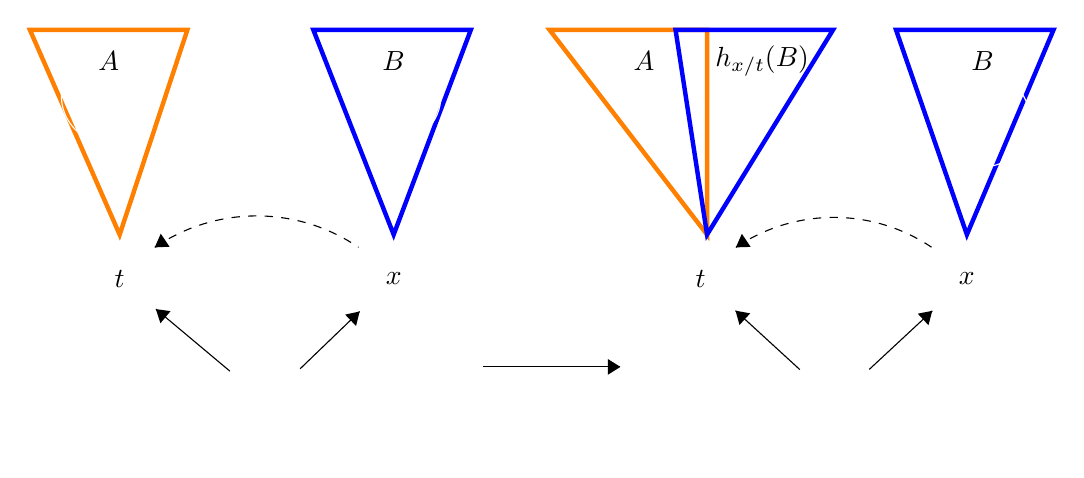
\begin{tikzpicture}[scale=0.2]
\tikzstyle{every node}+=[inner sep=0pt]
\draw [white] (20,-48.6) circle (3);
\draw [white] (10.7,-40.8) circle (3);
\draw (10.7,-40.8) node {$t$};
\draw[orange, ultra thick] (10.7,-38) -- (5,-25) -- (15,-25) -- cycle;
\draw [white] (28.1,-40.8) circle (3);
\draw (28.1,-40.8) node {$x$};
\draw[blue, ultra thick] (28.1,-38) -- (23,-25) -- (33,-25) -- cycle;
\draw [white] (10,-29.2) circle (3);
\draw (10,-27) node {$A$};
\draw [white] (28.1,-29.2) circle (3);
\draw (28.1,-27) node {$B$};
\draw [white] (56.1,-48.6) circle (3);
\draw [white] (47.6,-40.8) circle (3);
\draw (47.6,-40.8) node {$t$};
\draw[orange, ultra thick] (48,-38) -- (38,-25) -- (48,-25) -- cycle;
\draw[blue, ultra thick] (48,-38) -- (46,-25) -- (56,-25) -- cycle;
\draw [white] (64.5,-40.8) circle (3);
\draw (64.5,-40.8) node {$x$};
\draw[blue, ultra thick] (64.5,-38) -- (60,-25) -- (70,-25) -- cycle;
\draw (44,-27) node {$A$};
\draw (51.5,-27) node {$h_{x/t}(B)$};
\draw [white] (65.5,-30.7) circle (3);
\draw (65.5,-27) node {$B$};
\draw [white] (30.8,-46.4) circle (3);
\draw [white] (45.5,-46.4) circle (3);
\draw [black] (17.7,-46.67) -- (13,-42.73);
\fill [black] (13,-42.73) -- (13.29,-43.63) -- (13.93,-42.86);
\draw [black] (22.16,-46.52) -- (25.94,-42.88);
\fill [black] (25.94,-42.88) -- (25.02,-43.08) -- (25.71,-43.8);
\draw [black,dashed] (12.931,-38.807) arc (124.28182:55.71818:11.484);
\fill [black] (12.93,-38.81) -- (13.87,-38.77) -- (13.31,-37.94);
\draw [black] (53.89,-46.57) -- (49.81,-42.83);
\fill [black] (49.81,-42.83) -- (50.06,-43.74) -- (50.74,-43);
\draw [black] (58.3,-46.56) -- (62.3,-42.84);
\fill [black] (62.3,-42.84) -- (61.38,-43.02) -- (62.06,-43.75);
\draw [black,dashed] (49.831,-38.809) arc (124.01582:55.98418:11.116);
\fill [black] (49.83,-38.81) -- (50.77,-38.78) -- (50.21,-37.95);
\draw [black] (33.8,-46.4) -- (42.5,-46.4);
\fill [black] (42.5,-46.4) -- (41.7,-45.9) -- (41.7,-46.9);
\end{tikzpicture}
\end{center}
\label{figure:step1}
\caption{Illustration of the proof}
\end{figure}

Graphically, in the Figure \ref{proof}, if we note $A=\Tree_{F_m}(t)$ and $B=\Tree_{F_m}(x)$, then we want do an atomic merge derivation from the left factbase to the right factbase.


To prove the Proposition \ref{step1}, we will look all the triggers dealing with the variables in $\des(x)$ and apply them on the variables in $\des(t)$ if the triggers have not already been applied.

\begin{proof}
In order to define an atomic merge chase sequence such as $D'$, we first introduce some sequences of oblivious triggers:
\begin{itemize}
\item Let $t_1 = (\alpha_1,\sigma_1),\ldots, t_n =(\alpha_n,\sigma_n)$ be the maximal sequence of oblivious triggers such that:
(1) for each $1 \leq i \leq n$, there is some $1 \leq j \leq m$ such that $\Appl(F_j, t_i) = F_{j+1}$;
(2) if $F_k = \Appl(F_{k-1}, t_i)$ and $F_l = \Appl(F_{l-1},t_j)$ for some $i, j \in \{1, \ldots, n\}$ and  some $1 \leq k < l \leq m$, then $i<j$; and (3) the range of $\sigma_i$ is a subset of $\des(x)$ for each $1 \leq i \leq n$.
\item Let $t'_1, \ldots, t'_o$ be the maximal subsequence of $(\alpha_1, h_{x/t} \circ \sigma_1), \ldots, (\alpha_n, h_{x/t} \circ \sigma_n)$ such that $\Appl(F_{m}, t'_i) \neq F_{m}$ for each $1 \leq i \leq o$.
\end{itemize}

$t'_1, \ldots, t'_o$ are the triggers that \todo{}

Let $F_{m+i} = \Appl(F_{m+i-1}, t'_i)$ for each $1 \leq i \leq o$.
We show via induction that the sequence $D' = D, F_{m+1}, \ldots, F_{m+o}$ satisfies conditions 1. and 2. stated in the proposition.


For each $1 \leq i \leq n$, let $h_{x/t}(t_i) = (\alpha_i, h_{x/t} \circ \sigma_i)$.
Let $t_1, \ldots, t_r$ be the maximal subsequence of $h_{x/t}(t_1), \ldots, h_{x/t}(t_n)$ such that for all $i$, $\Appl(F_{m}, t_i) \neq F_{m}$.


We pose $F_{m+1} = \Appl(F_m,t_1),\ldots, F_{m+r} = \Appl(F_{m+r-1},t_r)$ and for $i \in \{1,\ldots,n\}$, $$B_i' = {h_{x/t} \circ \sigma_1^s}(Head(\alpha_1)) \cup \ldots \cup {h_{x/t} \circ \sigma^s_i}(Head(\alpha_{i}))$$

We note $D_0 = D$, $r(0) = 0$, and for $i \in \{1,\ldots,n\}$, if there exists $r(i) \in \{1,\ldots,r\}$ such that $h_{x/t}(tr_i) = t_{r(i)}$, then we note $D_i = D_{i-1},F_{m+r(i)}$; Otherwise, we note $D_i = D_{i-1}$ and we pose $r(i) = r(i-1)$. The integer $r(i)$, for $i >0$, verifie the condition $\Appl(F_{m+r(i)},tr_i) =  F_{m+r(i)}$.
\todo{I am getting lost around here; let's discuss it in the next meeting. <- I change a litle bit, is it better ?}

We show by induction on $i \in \{0,\ldots, n\},H(i)$: The sequence $D_i$ is an atomic merge chase and $B_i' \subseteq F_{m+r(i)}$. For i = 0, $D_0 = D$ is an oblivious derivation and $B_0' = \emptyset$, so $H(0)$ is true. Suppose that $H(i-1)$ is true for $i \in \{1,\ldots,n\}$.

If $\Appl(F_{m},h_{x/t}(tr_{i})) = F_{m}$ then $h_{x/t} \circ \sigma_i^s(Head(\alpha_i)) \subseteq F_{m+r(i)}$ so $B_i' = B_{i-1}' \cup h_{x/t} \circ \sigma_i^s(Head(\alpha_i)) 	\subseteq F_{m+r(i)}$. Therefore $D_i = D_{i-1}$ is suitable, $H(i)$ is true.

Otherwise, the oblivious trigger $h_{x/t}(tr_{i})$ has not been applied on $F_{m}$, there exists $j$ such that $h_{x/t}(tr_{i}) = t_j$. Depending on the form of the rule $\alpha_i$, there exists four different cases:
	\begin{itemize}
	\item If $\alpha_i$ is of the form $A(u) \rightarrow \exists v.R(u,v) \wedge B(v)$. We have $A(\sigma_i(u)) \in F_m$.
		\begin{itemize}
		\item If $\sigma_i(u) = x$, then $A(x) \in F_m$. As $t$ is a strong sibling of $x$ in $F_m$, $A(t) \in F_m$. So $A(h_{x/t}(\sigma_i(u))) \in F_{m+r(i-1)}$ since $h_{x/t}(\sigma_i(u)) = t$.  
		\item If $x \prec^+ \sigma_i(u)$, then the fact $A(\sigma_i(u)))$ is in $\sigma_j^s(Head(\alpha_j))$ where $j<i$. We have then $A(h_{x/t}(\sigma_i(u)))\in B_{i-1}'$ so by induction hypothesis, $A(h_{x/t}(\sigma_i(u)))\in F_{m+r(i-1)}$. 
		\end{itemize}
Therefore $h_{x/t}(tr_{i})$ is an oblivious trigger for $F_{m+r(i-1)}$.

	\item If $\alpha_i$ is of the form $A_1(u) \wedge A_2(u) \rightarrow B(u)$. We have $A_1(\sigma_i(u)),A_2(\sigma_i(u)) \in F_m$.
		\begin{itemize}
		\item If $\sigma_i(u) = x$, then $A_1(x),A_2(x) \in F_m$. As $t$ is a strong sibling of $x$ in $F_m$, we have $A_1(t),A_2(t) \in F_m$. So $A_1(h_{x/t}(\sigma_i(u))),A_2(h_{x/t}(\sigma_i(u))) \in F_{m+r(i-1)}$ since $h_{x/t}(\sigma_i(u)) = t$.  
		\item If $x \prec^+ \sigma_i(u)$, then the facts $A_1(\sigma_i(u)))$ and $A_2(\sigma_i(u)))$ are in $\sigma_j^s(Head(\alpha_j))$ where $j<i$. We have then $A_1(h_{x/t}(\sigma_i(u))),A_2(h_{x/t}(\sigma_i(u)))\in B_{i-1}'$ so by induction hypothesis, $A_1(h_{x/t}(\sigma_i(u))),A_2(h_{x/t}(\sigma_i(u)))\in F_{m+r(i-1)}$. 
		\end{itemize}
Therefore $h_{x/t}(tr_{i})$ is an oblivious trigger for $F_{m+r(i-1)}$.  

\item If $\alpha_i$ is of the form $A(u) \wedge R(u,v) \rightarrow B(v)$.
	\begin{itemize}
		\item If $\sigma_i(u) = x$, then $A(x) \in F_m$. As $t$ is a strong sibling of $x$ in $F_m$, $A(t)\in F_m$. Thus $A(h_{x/t}(\sigma_i(u))) \in F_{m+r(i-1)}$.
		\item If $x \prec^+ \sigma_i(u)$, then the fact $A(\sigma_i(u)))$ is in $\sigma_j^s(Head(\alpha_j))$ where $j<i$. We have then $A(h_{x/t}(\sigma_i(u)))\in B_{i-1}'$ so by induction hypothesis, $A(h_{x/t}(\sigma_i(u)))\in F_{m+r(i-1)}$. 
		\end{itemize}
The fact $R(\sigma_i(u),\sigma_i(v))$ is in $\sigma_j^s(Head(\alpha_j))$ where $j<i$. We have then $R(h_{x/t}(\sigma_i(u)),h_{x/t}(\sigma_i(v)))\in B_{i-1}'$ so by induction hypothesis, $R(h_{x/t}(\sigma_i(u)),h_{x/t}(\sigma_i(v)))\in F_{m+r(i-1)}$. 		

Therefore, the facts $A(h_{x/t}(\sigma_i(x)))$ and $R(h_{x/t}(\sigma_i(u)),h_{x/t}(\sigma_i(v)))$ are in $ F_{m+r(i-1)}$. Thus $h_{x/t}(tr_{i})$ is an oblivious trigger for $F_{m+r(i-1)}$.
\item If $\alpha_i$ is of the form $R(u,v) \wedge B(v) \rightarrow A(u)$. $\sigma_i(u) \neq x$ since $A(t) \in F_{m}$

The facts $R(\sigma_i(u),\sigma_i(v)),B(\sigma_i(v))$ have been introduced by oblivious triggers in $\{tr_1,\ldots,tr_{i-1}\}$. So, by induction hypothesis, the facts $R(h_{x/t}(\sigma_i(u)),h_{x/t}(\sigma_i(v)))$ and $B(h_{x/t}(\sigma_i(v)))$ are in $ F_{m+r(i-1)}$. Therefore $h_{x/t}(tr_{i})$ is an oblivious trigger for $F_{m+r(i-1)}$.
\item If $\alpha_i$ is of the form $R_1(u,v) \wedge R_2(u,v) \rightarrow S(u,v)$.

The facts $R_1(\sigma_i(u),\sigma_i(v)),R_2(\sigma_i(u),\sigma_i(v))$ are in $\sigma_j^s(Head(\alpha_j))$ where $j<i$. We have then $R_1(h_{x/t}(\sigma_i(u)),h_{x/t}(\sigma_i(v))),R_2(h_{x/t}(\sigma_i(u)),h_{x/t}(\sigma_i(v)))\in B_{i-1}'$ so by induction hypothesis, $R_1(h_{x/t}(\sigma_i(u)),h_{x/t}(\sigma_i(v))),R_2(h_{x/t}(\sigma_i(u)),h_{x/t}(\sigma_i(v)))\in F_{m+r(i-1)}$. 



	\end{itemize} 

As $h_{x/t}(tr_{i})$ is an oblivious trigger for $F_{m+r(i-1)}$, $D_i$ is an atomic merge derivation. By definition of an application, we have $h_{x/t} \circ \sigma_i^s(Head(\alpha_i)) \subseteq F_{m+r(i)}$ and so $B_i' = B_{i-1} \cup h_{x/t} \circ \sigma_i^s(Head(\alpha_i)) 	\subseteq F_{m+r(i)}$.
Therefore, $H(i)$ is true.


We have proved the heredity. So, $D_n$ is the oblivious derivation that we was looking for. We have $F_{m+k} = F_m \cup h_{x/t}(\Tree_{F_m}(x))$.

\end{proof}




\begin{proposition} \label{step2}
Let $D = F_0,trig_1,F_1,\ldots, trig_m,F_m$ be an atomic merge chase derivation for the knowledge base $K$. Assume that $x$ is mergeable on $t$ in $F_m$, the atomic merging of $x$ on $t$ in $F_m$ is a retract of $\Fut(F_m,t,x)$ .
\end{proposition}

\begin{proof}
The atomic merging of $x$ on $t$ in $F_m$ is $h_{x/t}(F_m)$. By the Proposition \ref{step1}, $\Fut(F_m,t,x)= F_m \cup h_{x/t}(\Tree_{F_m}(x))$. So, $h_{x/t}(F_m) \subseteq \Fut(F_m,t,x) $ since $\Fut(F_m,t,x) = \Tree_{F_m}(x) \cup h_{x/t}(F_m)$. Finally, as $h_{x/t}(\Fut(F_m,t,x)) = h_{x/t}(F_m)$, we have that $h_{x/t}(F_m) \models \Fut(F_m,t,x)$.
\end{proof}

The following theorem is a corollary of Propositions \ref{step1} and \ref{step2} :

\begin{theorem} \label{universality atomic merge}
When applied to a factbase in an atomic merge chase sequence, the atomic merge operation preserves universality.\todo{I would simply say that each fact set in an atomic merge sequence is universal. -> I define what mean that an operation preserve the universality and what are the properties at the end of thd part 2}
\end{theorem}

\begin{proof}
Let $K$ be a \ALCH\ knowledge base, $D=F_0,\ldots, F_m$ be an atomic merge chase derivation, and $M$ be a model of $K$ such that $M \models F_m$. Suppose that there exists a variable $x$ mergeable on a term $t$ in $F_m$. According to Proposition \ref{step1}, The factbase $\Fut(F_m,t,x)$ has been obtained from $F_m$ only by the use of the application operation. The Proposition  says that this operation preserves the universality. We have then $M \models \Fut(F_m,t,x)$. So $M$ is a model of the atomic merging of $x$ on $t$ in $F_m$ since, by Proposition \ref{step2}, it is a subset of $\Fut(F_m,t,x)$.
\end{proof}





The merge operation uses only atomic merge, so by Theorem \ref{universality atomic merge}:

\begin{theorem} \label{universality merge}
When applied to a factbase in an atomic merge chase sequence, the merge operation preserves universality.\todo{I think that it would be clearer to say that all of the elements in a merge sequence are universal.}
\end{theorem}


The main reason to prefer the merge chase instead of the atomic merge chase is that unless the atomic merging operations are applied exhaustively, the merge chase may not terminate on inputs that admit finite universal models:


\begin{theorem} \label{necessity of atomic merge}
There exists a \ALCH\ knowledge base and an infinite atomic merge chase derivation for $K$ such that $K$ admits a finite universal model.
\end{theorem}

\begin{figure}
\begin{center}
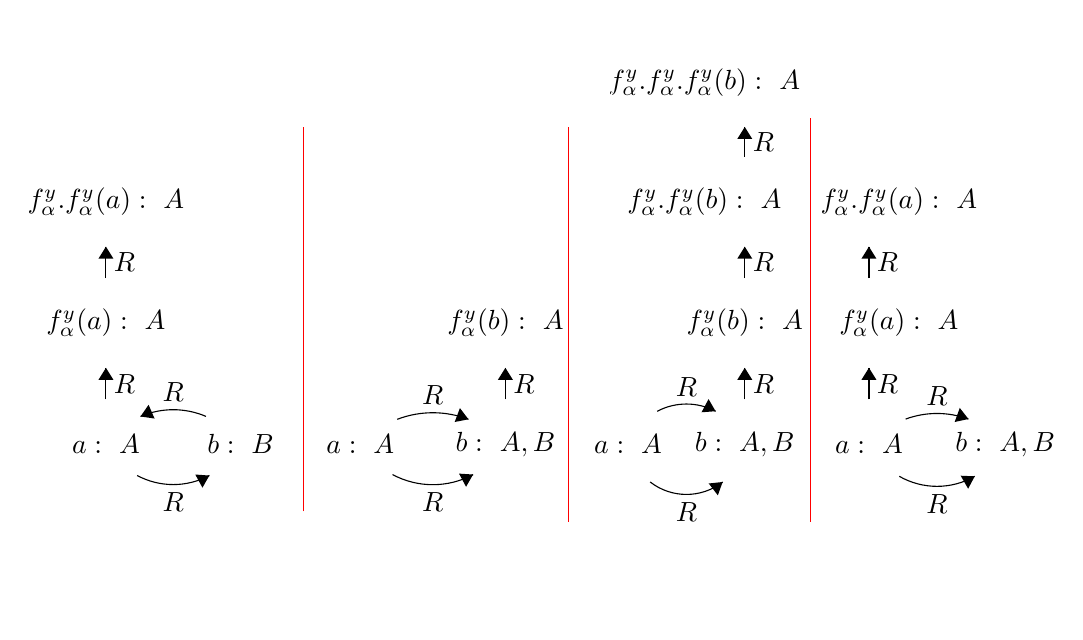
\begin{tikzpicture}[scale=0.19]
\tikzstyle{every node}+=[inner sep=0pt]
\draw [white] (16,-25.6) circle (3);
\draw (16,-25.6) node {$b:\mbox{ }B$};
\draw [white] (7,-25.6) circle (3);
\draw (7,-25.6) node {$a:\mbox{ }A$};
\draw [white] (7,-17.5) circle (3);
\draw (7,-17.5) node {$f_\alpha^y(a):\mbox{ }A$};
\draw [white] (7,-9.4) circle (3);
\draw (7,-9.4) node {$f_\alpha^y.f_\alpha^y(a):\mbox{ }A$};
\draw [white] (24,-25.6) circle (3);
\draw (24,-25.6) node {$a:\mbox{ }A$};
\draw [white] (33.7,-25.6) circle (3);
\draw (33.7,-25.6) node {$b:\mbox{ }A,B$};
\draw [white] (41.9,-25.6) circle (3);
\draw (41.9,-25.6) node {$a:\mbox{ }A$};
\draw [white] (49.7,-25.6) circle (3);
\draw (49.7,-25.6) node {$b:\mbox{ }A,B$};
\draw [white] (58,-25.6) circle (3);
\draw (58,-25.6) node {$a:\mbox{ }A$};
\draw [white] (67.1,-25.6) circle (3);
\draw (67.1,-25.6) node {$b:\mbox{ }A,B$};
\draw [white] (33.7,-17.5) circle (3);
\draw (33.7,-17.5) node {$f_\alpha^y(b):\mbox{ }A$};
\draw [white] (49.7,-17.5) circle (3);
\draw (49.7,-17.5) node {$f_\alpha^y(b):\mbox{ }A$};
\draw [white] (49.7,-9.4) circle (3);
\draw (47,-9.4) node {$f_\alpha^y.f_\alpha^y(b):\mbox{ }A$};
\draw [white] (49.7,-1.4) circle (3);
\draw (47,-1.4) node {$f_\alpha^y.f_\alpha^y.f_\alpha^y(b):\mbox{ }A$};
\draw [white] (58,-17.5) circle (3);
\draw (60,-17.5) node {$f_\alpha^y(a):\mbox{ }A$};
\draw [white] (58,-9.4) circle (3);
\draw (60,-9.4) node {$f_\alpha^y.f_\alpha^y(a):\mbox{ }A$};
\draw [white] (20.2,-33.1) circle (3);
\draw [white] (20.2,-1.4) circle (3);
\draw [white] (37.9,-33.8) circle (3);
\draw [white] (37.9,-1.4) circle (3);
\draw [white] (54.1,-33.8) circle (3);
\draw [white] (54.1,-0.8) circle (3);
\draw [black] (13.913,-27.695) arc (-61.74408:-118.25592:5.098);
\fill [black] (13.91,-27.7) -- (12.97,-27.63) -- (13.45,-28.51);
\draw (11.5,-28.8) node [below] {$R$};
\draw [black] (9.313,-23.747) arc (113.21358:66.78642:5.549);
\fill [black] (9.31,-23.75) -- (10.25,-23.89) -- (9.85,-22.97);
\draw (11.5,-22.8) node [above] {$R$};
\draw [black] (31.542,-27.634) arc (-61.78869:-118.21131:5.695);
\fill [black] (31.54,-27.63) -- (30.6,-27.57) -- (31.07,-28.45);
\draw (28.85,-28.81) node [below] {$R$};
\draw [black] (48.224,-28.129) arc (-52.06714:-127.93286:3.943);
\fill [black] (48.22,-28.13) -- (47.29,-28.23) -- (47.9,-29.02);
\draw (45.8,-29.46) node [below] {$R$};
\draw [black] (65.072,-27.751) arc (-60.23294:-119.76706:5.079);
\fill [black] (65.07,-27.75) -- (64.13,-27.71) -- (64.63,-28.58);
\draw (62.55,-28.92) node [below] {$R$};
\draw [black] (26.469,-23.941) arc (110.98089:69.01911:6.65);
\fill [black] (31.23,-23.94) -- (30.66,-23.19) -- (30.31,-24.12);
\draw (28.85,-23) node [above] {$R$};
\draw [black] (43.847,-23.403) arc (117.88071:62.11929:4.176);
\fill [black] (47.75,-23.4) -- (47.28,-22.59) -- (46.81,-23.47);
\draw (45.8,-22.42) node [above] {$R$};
\draw [black] (60.451,-23.924) arc (110.20979:69.79021:6.075);
\fill [black] (64.65,-23.92) -- (64.07,-23.18) -- (63.73,-24.12);
\draw (62.55,-23.05) node [above] {$R$};
\draw [black] (7,-22.6) -- (7,-20.5);
\fill [black] (7,-20.5) -- (6.5,-21.3) -- (7.5,-21.3);
\draw (7.5,-21.55) node [right] {$R$};
\draw [black] (7,-14.5) -- (7,-12.4);
\fill [black] (7,-12.4) -- (6.5,-13.2) -- (7.5,-13.2);
\draw (7.5,-13.45) node [right] {$R$};
\draw [black] (33.7,-22.6) -- (33.7,-20.5);
\fill [black] (33.7,-20.5) -- (33.2,-21.3) -- (34.2,-21.3);
\draw (34.2,-21.55) node [right] {$R$};
\draw [black] (49.7,-22.6) -- (49.7,-20.5);
\fill [black] (49.7,-20.5) -- (49.2,-21.3) -- (50.2,-21.3);
\draw (50.2,-21.55) node [right] {$R$};
\draw [black] (49.7,-14.5) -- (49.7,-12.4);
\fill [black] (49.7,-12.4) -- (49.2,-13.2) -- (50.2,-13.2);
\draw (50.2,-13.45) node [right] {$R$};
\draw [black] (49.7,-6.4) -- (49.7,-4.4);
\fill [black] (49.7,-4.4) -- (49.2,-5.2) -- (50.2,-5.2);
\draw (50.2,-5.4) node [right] {$R$};
\draw [black] (58,-22.6) -- (58,-20.5);
\fill [black] (58,-20.5) -- (57.5,-21.3) -- (58.5,-21.3);
\draw (58.5,-21.55) node [right] {$R$};
\draw [black] (58,-14.5) -- (58,-12.4);
\fill [black] (58,-12.4) -- (57.5,-13.2) -- (58.5,-13.2);
\draw (58.5,-13.45) node [right] {$R$};
\draw [red] (37.9,-30.8) -- (37.9,-4.4);

\draw [red] (20.2,-30.1) -- (20.2,-4.4);

\draw [red] (54.1,-30.8) -- (54.1,-3.8);

\end{tikzpicture}
\end{center}
\label{figure:atomic merge chase not efficient}
\caption{Example where the atomic merge chase is not efficient}
\end{figure}


\begin{proof} 
Let $F= \{R(a,b),R(b,a),A(a),A(b)\}$ and $R = \{\alpha = A(x) \rightarrow \exists y.R(x,y) \wedge A(y), \beta = B(x) \rightarrow A(x)\}$. We consider the atomic merge chase derivation for $K=(R,F)$ $F_0 =F,F_1,F_2,...$
\begin{itemize}

\item We applied to $F_0$ the oblivious trigger $t_1 = (\alpha, \{x \mapsto a\})$;
\item we then applied to $F_1$, the oblivious trigger $t_2 = (\alpha, \{x \mapsto f_\alpha^y(a)\})$ giving rise to the first factbase of the Figure \ref{figure:atomic merge chase not efficient};
\item we then apply the oblivious trigger $t_3 = (\beta, \{x \mapsto b\})$ to obtain the factbase $F_3$;
\item At this moment, $f_\alpha^y(a)$ is mergeable on $b$ so we do an atomic merging of $f_\alpha^y(a)$ on $b$ to get $F_4$ that is the second factbase of the figure;
\item $F_5$ is obtained by the application of the oblivious trigger $t_4 = (\alpha, \{x \mapsto f_\alpha^y(b)\})$ and $F_6$ by the oblivious trigger $t_5 = (\alpha, \{x \mapsto f_\alpha^y(f_\alpha^y(b))\})$, $F_6$ is the third factbase of the figure;
\item At this moment, $f_\alpha^y(b)$ is mergeable on $a$ so we do an atomic merging of $f_\alpha^y(b)$ on $a$ to get $F_7$ that is the last factbase of the figure; 
\item We can repeat this infinitely. 

\end{itemize} 
 But $K$ admits a finite universal model: $U = F \cup \{B(b)\}$. 

\todo{Improve write-up; discuss. is it better ?}



\end{proof}



We want now prove that a merging computes a core:

\begin{proposition} \label{core}
For a factbase $G$ that occurs in a merge chase derivation of some \ALCH\ knowledge base, $\Merge(G)$ is a core.
\end{proposition}

\begin{proof}
%\item The $\mathcal{ALCH}$-pruning algorithm only take off facts of the factbase. Consequently, $\textit{prune}(G) \subseteq G$.
%\item We consider the homorphism $h:G \to \textit{prune}(G)$ created during the $\mathcal{ALCH}$-pruning algorithm. For $x \in \Vars(G)$, suppose that $h(x) \neq x$. According to the $\mathcal{ALCH}$-pruning algorithm, $x$ has been erased \todo{à préciser}. So $x \notin \Vars(\textit{prune}(G))$. So ${h}_{|\textit{Prune}(G)}=id_{|\textit{Prune}(G)}$. We have shown that $h$ is a retract so $\textit{prune}(G)$ is a retract of $G$.
Suppose for a contradiction that $\Merge(G)$ is not a core. There exists a factbase $G' \subsetneq \Merge(G)$ such that $G'$ is a retract of $\Merge(G)$. By Proposition \ref{retract}, there exists then a retractation $h$ from $\Merge(G)$ to $G'$. We have $var(\Merge(G))\setminus var(G') \neq \emptyset$. Let $x$ be a $\prec$-minimal variable of this set. The term $x$ is a variable, so has been introduced by the chase due to a rule of the form \ref{rule:horn-alc-exist}. So there exists a term $t$ such that $t \prec x$. 
\begin{itemize}
\item We have $\Preds^2_{\Merge(G)}(t,x) \neq \emptyset$. By $\prec$-minimality of $x$, $t \in \Vars(G')$. So, as $h$ is a retractation: $h(t) = t$, so for $R \in \Preds^2_{\Merge(G)}(t,x)$, $h(R(t,x)) = R(t,h(x)) \in \Merge(G)$ and so $R \in \Preds^2_{\Merge(G)}(t,h(x))$. Thus $\Preds^2_{\Merge(G)}(t,x) \subseteq \Preds^2_{\Merge(G)}(t,h(x))$ and $t \prec h(x)$.
\item $x \notin G'$ and $h(x) \in G'$ so $h(x) \neq x$. 
\item Let $A \in \Preds^1_{\Merge(G)}(x)$. $h(A(x)) \in \Merge(G)$ so $A(h(x)) \in \Merge(G)$ so $\Preds^1_{\Merge(G)}(x) \subseteq \Preds^1_{\Merge(G)}(h(x))$. 
\end{itemize}
Consequently, $x$ is mergeable on $h(x)$ in $\Merge(G)$ which results on a contradiction. Hence, $\Merge(G)$ is a core.
\end{proof}	

$\Merge(G)$ is a core but not necessarily the core of $G$.


%\begin{definition}
%$tr = (\alpha,\sigma, \hat \sigma)$ is a \emph{stupid trigger} if $(\alpha,\sigma)$ is an oblivious trigger, and if $\hat \sigma$ extends $\sigma$ and is defined on $\Vars(\textit{Head}(\alpha))$. The factbase $\Appl(F,tr)=F \cup \hat \sigma(\textit{Head}(\alpha))$ is called an \emph{application} on the factbase $F$ through the stupid trigger $tr = (\alpha,\sigma, \hat \sigma)$. A \emph{stupid derivation} from a knowledge base $K= (F,R)$ is a (possibly infinite) sequence $D=F_0,tr_1,F_1,tr_2,F_2,\ldots$ where $(F_i)_{i \in \N}$ are factbases, $tr_i$ are stupid triggers, $F_0 = F$, and for $i >0$, $F_{i}= \Appl(F_{i-1},tr_i)$ is obtained by an application. The stupid derivation $D=F_0,t_1,F_1,t_2,F_2,\ldots$ is \emph{fair} if for every $i$ and every stupid trigger $tr = (\alpha,\sigma, \hat \sigma)$ applicable on $F_i$, there exists $k \geq i$ such that there exists a stupid trigger $tr' = (\alpha,\sigma, \hat \sigma')$ that verified $\Appl(F_{k},tr') = F_k$. A \emph{stupid chase} for a knowledge base $K= (F,R)$ is a fair stupid derivation $D=F_0,tr_1,F_1,tr_2,F_2,\ldots$ $F_0 \subseteq F_1 \subseteq F_2 \subseteq \ldots$ so we can pose \emph{$\textit{Stp(K)}$} = $\cup_{i \in \N}F_i$.
%We say that the stupid chase \emph{terminates} if $\textit{Stp(K)}$ is finite.
%\end{definition}




\begin{proposition} \label{finite <- terminates}
The merge chase computes a finite universal model of $K$ when it terminates.
\end{proposition}

\begin{proof}
Let $D = F_0,\ldots,F_n$ be a merge chase for $K =(R,G)$. 
\begin{itemize}
\item The merge chase never take off ground facts and $G =F_0$ so $G \subseteq F_n$. We have then $F_n \models G$. Assume for a contradiction that $F_n \nvDash R$. There exists then a rule $\alpha$ in $R$ not satisfied by $F_n$: $F_n \vDash \textit{Body}(\alpha)$ and $F_n \nvDash \textit{Head}(\alpha)$. It means that there exists a substitution $\sigma$ from $\textit{Body}(\alpha)$ to $F_n$. Therefore, $t=(\alpha,\sigma)$ is an oblivious trigger for $F_n$. As the derivation $D$ is fair, there exists $k$ such that $\Appl(F_k,t) = F_k$. Thus $\sigma^s(\textit{Head}(\alpha)) \subseteq F_k$, so $F_k \models \alpha$. As $F_n \models F_k$, $F_n \models \alpha$ which lead us to a contradiction. We have then $F_n \models R$ so $F_n$ is a model of $K$.
\item According to Proposition \ref{universality application} and \ref{universality merge}, each operation of the merge chase conserves the universality so we can show by induction that $F_n$ is a universal model of $K$.
\item $F_n$ is finite.
\end{itemize}
\end{proof}

\begin{proposition} \label{finite -> terminates}
If there exists a finite universal model for a \ALCH\ knowledge base $K = (R,F)$, then the merge chase terminates.
\end{proposition}

\begin{proof}
\begin{itemize}
\item Suppose for a contradiction that $K$ admits a finite universal model $U$ for $K$ and does not admit a finite merge chase sequence. There exists so an infinite merge chase sequence $D= F_0, F_2, \ldots$
\item A term $t$ is \emph{redundant} with respect to this sequence if $t \in \Terms(F_i)$ and $t \notin \Terms(F_j)$ for some $i < j$.
\item For each $i$, let $G_i$ be the maximal subset of $F_i$ that does not contain redundant terms.

\item We pose $M = \cup_i~G_i$. For a model $N$ of $K$ and for $i \in \N$, there exits a homomorphism $h_i$ from $F_i$ to $N$ since $F_i$ is universal for $K$ by Proposition \ref{universality merge}. As $G_i \subseteq F_i$, $h_i$ is a homomorphism from $G_i$ to $N$. Finally, $\cup_i~h_i$ is a homomorphism from $M$ to $N$ so $M$ is universal for $K$.

\item Constants cannot be redondants, so $F \subseteq M$ since $G_0 =F$. We have then $M \vDash F$. Assume for a contradiction that $M \nvDash R$. There exists then a rule $\alpha$ in $R$ not satisfied by $M$: $M \vDash \textit{Body}(\alpha)$ and $M \nvDash \textit{Head}(\alpha)$. As $D$ is fair, there exists $k$ such that $F_k \vDash \textit{Head}(\alpha)$. For a homomorphism $\sigma$ from $\textit{Head}(\alpha)$ to $F_k$, there exists then a redundant term $t$ in the domain of $\sigma^s$. Thus, by definition of a redundant term, there exists $l > k$ such that $t \notin \Terms(F_l)$ 


It means that there exists a substitution $\sigma$ from $\textit{Body}(\alpha)$ to $F_n$. Therefore, $t=(\alpha,\sigma)$ is an oblivious trigger for $F_n$.

It is an universal model of $K$ so $M \models U$. There exists then a homomorphism $h$ from $U$ to $M$. As $U$ is finite, the factbase $h(U)\subseteq M$ is also finite. The sequence $G_0,G_1,\ldots$ is monotonic (that is $G_0 \subseteq G_1 \subseteq \cdots$) so there exist $i$ such that $h(U) \subseteq G_i$. We have then $F_i \models h(U)$ since $G_i \subseteq F_i$. We have $h(U) \models U$, so $F_i\models U$. As all the used operations during a merge chase preserves the universality and as $U \models F_0$, $U \models F_i$. Therefore $F_i$ is a finite universal model for $K$.

\item There exists a finite number of triggers for $F_i$ and $D$ is fair. So, there exists $j \geq i$ such that all the triggers for $F_i$ has been applied in the derivation $F_0,F_1,\ldots,F_j$.

\item As $D$ is fair, there exists $k \geq j$ such that $F_k$ is a core. We have $F_k \subseteq F_i$ so all the triggers for $F_k$ has been applied in the derivation $F_0,F_1,\ldots,F_k$.
\item The derivation $F_0,\ldots,F_k$ is therefore fair so it is a finite merge chase sequence which leads us to a contradiction.
\end{itemize}
\todo{This proof needs a bit more work; do you have any questions about it?}
\end{proof}

The following theorem is then a direct consequence of Propositions \ref{finite <- terminates} and \ref{finite -> terminates}.

\begin{theorem}
The merge chase computes an universal model if and only if there exists an universal model.
\end{theorem}

We will now describe a deterministic algorithm to merge a factbase:

\begin{definition}[Merging]
Let $F$ be a factbase that occurs in a merge chase derivation of the knowledge base $K$.

\begin{algorithm}[H] \label{algo}
\SetAlgoLined


    Let $\textbf{\Vars}(F) = \{x_1,\ldots, x_n\}$ be such that $(x_i \prec^+ x_j) \Rightarrow i < j$ \;
    \For{$i =1 \text{ to } n$}{
    	\If{$x_i$ is still a variable in $F$}{
			\For{all term $t$ such that $x_i$ is mergeable on $t$}{
				$F \leftarrow$ the atomic merging of $x_i$ on $t$ in $F$.
			}
		}
	}
return $F$
\caption{Merge($F$):}


\end{algorithm}
At line 1, we can sort terms like that because, by proposition \ref{partial_order}, $\prec^+$ is a strict partial order over the set of variables of $F$.
\end{definition}



Note that the application of an atomic merge may result in new mergeable variables. Therefore, we have to be carefull about the order of the variables in the Algorithm \ref{algo}. In the Example \ref{example: merging}, if we treat $f_\beta^z(f_\alpha^z(a))$ before $f_\alpha^z(a)$, then at the moment where we treat $f_\beta^z(f_\alpha^z(a))$, it does not have any term $t$ yet such that $f_\beta^z(f_\alpha^z(a))$ is mergeable on $t$. At the end, we get the factbase of the middle and we will not have merged every possible mergeable variable.


The Example \ref{necessity of atomic merge} shows the importance of doing a total merging. We have to prove that our merging algorithm does a total merging:

\begin{proposition}\label{no_more_siblings}
Let $G$ be a factbase that occurs in a chase derivation of the knowledge base $K$. There does not exists a term $t$ and a variable $x$ such that $x$ is mergeable on $t$ in $\Merge(G)$.
\end{proposition}

\begin{proof} 
Suppose for a contradiction that there exists a term $t$ and a variable $x$ such that $x$ is mergeable on $t$ in $\Merge(G)$, that is, there exists a term $t'$ such that $\Preds^2_{\Merge(G)}(t',x) \neq \emptyset$ and $\Preds_{\Merge(G)}^2(t',x) \subseteq \Preds_{\Merge(G)}^2(t',t)$. This case can happen only if $x$ became mergeable after that $x$ has been traited by the merging algorithm. Thus, during the merging, there has been an atomic merging on $t'$. Let $y$ be the variable merged on $t'$ such that $y \prec x$. We note $G^1$ the factbase just before the atomic merging of $y$ on $t'$ and we note $G^2$ the factbase just after the atomic merging. There exists a term $t_0$ such that $\Preds^2_{G^1}(t_0,y) \neq \emptyset$ and $\Preds_{G^1}^2(t_0,y) \subseteq \Preds_{G^1}^2(t_0,t')$. The factbase $G^1$ is in the left of the Figure \ref{figure:proof} and the factbase $G^2$ is in the right (we do not represent all the graphs):

\begin{figure}
\begin{center}
\begin{tikzpicture}[scale=0.2]
\tikzstyle{every node}+=[inner sep=0pt]
%\filldraw[color=red!60, fill=red!5, very thick](17,-38) circle (6);
%\filldraw[color=red!60, fill=red!5, very thick](60,-39) circle (6);
%\filldraw[color=red!60, fill=red!5, very thick](10,-11) circle (4);
%\filldraw[color=red!60, fill=red!5, very thick](25,-11) circle (4);
%\filldraw[color=red!60, fill=red!5, very thick](65,-11) circle (4);
%\filldraw[color=red!60, fill=red!5, very thick](54,-11) circle (4);
\draw [white] (17.1,-35.9) circle (3);
\draw (17.1,-35.9) node {$t_0$};
\draw [white] (10.1,-24.1) circle (3);
\draw (10.1,-24.1) node {$t'$};
\draw [white] (24.1,-24.1) circle (3);
\draw (24.1,-24.1) node {$y$};
\draw [white] (24.1,-12.4) circle (3);
\draw (24.1,-12.4) node {$x$};
\draw [white] (10.1,-12.4) circle (3);
\draw (10.1,-12.4) node {$t$};
\draw [white] (30.7,-24.6) circle (3);
\draw [white] (50.4,-24.6) circle (3);
\draw [white] (59.7,-36.8) circle (3);
\draw (59.7,-36.8) node {$t_0$};
\draw [white] (59.7,-25.3) circle (3);
\draw (59.7,-25.3) node {$t'$};
\draw [white] (53.4,-13.2) circle (3);
\draw (53.4,-13.2) node {$t$};
\draw [white] (65.4,-13.2) circle (3);
\draw (65.4,-13.2) node {$x$};
\draw [black] (15.57,-33.32) -- (11.63,-26.68);
\fill [black] (11.63,-26.68) -- (11.61,-27.62) -- (12.47,-27.11);

\draw [black] (10.1,-21.1) -- (10.1,-15.4);
\fill [black] (10.1,-15.4) -- (9.6,-16.2) -- (10.6,-16.2);

\draw [black] (18.63,-33.32) -- (22.57,-26.68);
\fill [black] (22.57,-26.68) -- (21.73,-27.11) -- (22.59,-27.62);

\draw [black] (24.1,-21.1) -- (24.1,-15.4);
\fill [black] (24.1,-15.4) -- (23.6,-16.2) -- (24.6,-16.2);

\draw [black] (33.7,-24.6) -- (47.4,-24.6);
\fill [black] (47.4,-24.6) -- (46.6,-24.1) -- (46.6,-25.1);
\draw [black] (59.7,-33.8) -- (59.7,-28.3);
\fill [black] (59.7,-28.3) -- (59.2,-29.1) -- (60.2,-29.1);

\draw [black] (58.31,-22.64) -- (54.79,-15.86);
\fill [black] (54.79,-15.86) -- (54.71,-16.8) -- (55.6,-16.34);

\draw [black] (60.98,-22.59) -- (64.12,-15.91);
\fill [black] (64.12,-15.91) -- (63.33,-16.42) -- (64.23,-16.85);

\end{tikzpicture}
\end{center}
\label{figure:proof}
\caption{Illustration of the proof}
\end{figure}

We have $t_0 \prec t' \prec t$ and $t_0 \prec y \prec x$ so $x$ should have been treated by the algorithm after the merging of $t'$ and $y$ so the algorithm will merge $x$ on $t$. It is a contradiction. 
\end{proof}


\subsection{\ALCHI}

\begin{definition}[\ALCHI\ axioms]
A \emph{\ALCHI\ axiom} is either a \ALCH\ axiom or an existential rule of the form:
\begin{align}
R_1(x,y) \wedge R_2(x,y) \rightarrow S(y,x)
\end{align}

A \emph{\ALCHI\ knowledge base} $K = (R,F)$ is a knowledge base where $R$ is a set of \ALCHI\ axioms and $F$ contains only predicates of arity one or two. 

\end{definition}

We have to modify the merge chase because it does not work anymore:

We keep the same relation $\prec$. It is still a strict partial order over the set of variables.



\bibliographystyle{plain}
\bibliography{sample}


\end{document}